\title{Enhancing EDA and Misclassification Analysis through Tree Structure Visualization}
\author{
        Maor Hornstein \\
        \small{Tabular Data Science (89547) - Final Project}\\
}
\date{}

\documentclass[12pt]{article}
\usepackage{graphicx}
\usepackage{caption}
\usepackage{refstyle}
\usepackage{xcolor}
\usepackage[labelsep=quad,indention=10pt]{subfig}
\usepackage[export]{adjustbox}
\usepackage{multirow}
\usepackage{array}
\newcolumntype{P}[1]{>{\centering\arraybackslash}p{#1}}

\DeclareCaptionFont{gray}{\color{gray}}
\usepackage[font={color=gray}]{caption}

\renewcommand{\arraystretch}{1.5}

\begin{document}
\maketitle

\begin{abstract}
a short summary of the problem, your solution, and experimental results (up to 200 words).
\end{abstract}

\section{Problem Description}\label{Problem Description}
The focus of the solution is on the Exploratory Data Analysis (EDA) phase, particularly the use of scatter plots in this phase.

Scatter plots are a useful tool in data analysis and visualization due to their simplicity and ability to show the relationship between two or more groups. They are easy to comprehend and interpret, making them accessible for people with diverse backgrounds. Scatter plots help to uncover trends, patterns and outliers, examine the interactions between variables, and to highlight significant aspects of the data

Despite their usefulness, scatter plots have some limitations. For instance, when data points are tightly packed or overlap (often referred to as overplotting), it can be challenging to accurately gauge the actual density of the data. Another significant challenge is distinguishing between groups when they overlap or when there is a small sample size. Lastly, Scatter plot only displays the distribution of the data in two dimensions and does not give insights into density or distribution in additional dimensions.

\section{Solution overview - The ICC plot}\label{Solution overview}
The proposed solution is a tree-based representation offered as an alternative to scatter plots to address their limitations.

The tree structure mimics the process a researcher goes through when analyzing a scatter plot, visually dividing the plane into subplanes and examining the density and distribution of samples in each subplane, as illustrated in \figref{fig1}.

\begin{figure}[h]
\centering
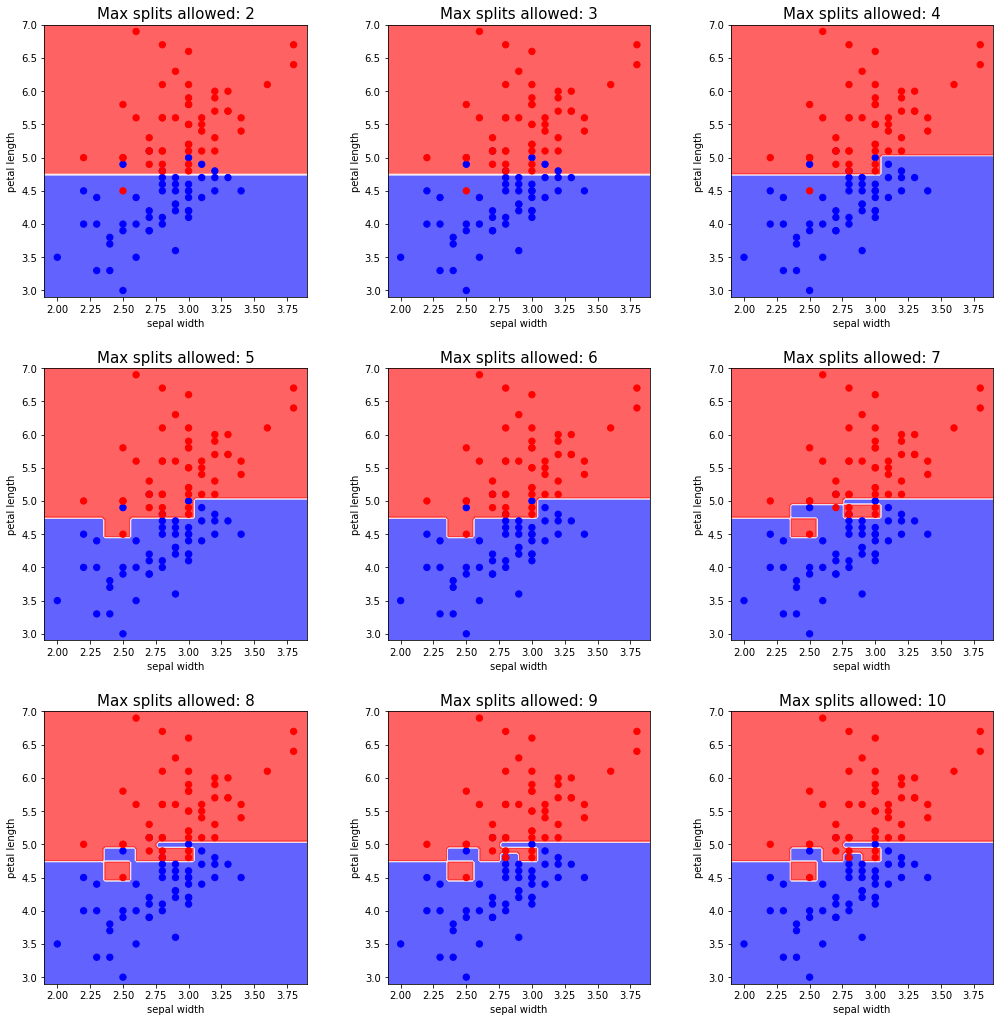
\includegraphics[width=0.8\textwidth]{scatter_plot_illustration.png}

\caption{Illustrates how a researcher visually divides the Scatter plot if he or she uses only horizontal and vertical lines. The simulation is based on a subset of the Iris dataset containing only the Versicolor and Virginica classes and the Sepal width and Petal length attributes.}
\label{fig:fig1}

\end{figure}

The selection of a tree structure representation was inspired by the widespread use of trees in daily decision making. Also, unlike the scatter plots that only feature points, a tree enables additional information to be displayed at its vertices and arcs. Last, the branching structure of the tree facilitates the analysis of multiple dimensions of the data.

Visual features such as colors and gradients aid in emphasizing the data's distribution, while confusion matrices at the tree nodes depict precisely the data's density.

I named the representation ICC plot, as an acronym of its 3 components: \textbf{I}nduction tree, \textbf{C}onfusion matrices and \textbf{C}olors.

\begin{figure}[h]
\centering
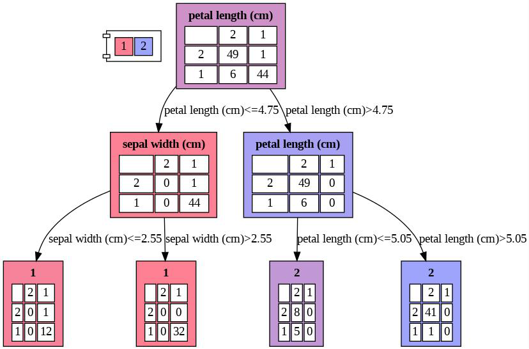
\includegraphics[width=0.8\textwidth]{icc.png}

\caption{ICC with 3 nodes simulate a plain with 3 splits.}
\label{fig:fig2}

\end{figure}

The ICC offers additional functionality to the researcher, such as adjusting the tree depth to increase or decrease the number of simulated splits of the plain, hiding the confusion matrices to focus on the data spread instead of specific quantities, and adjusting colors, as illustrated in  \figref{fig3}.

\begin{figure}[h]
        	\centering
           \subfloat{%
              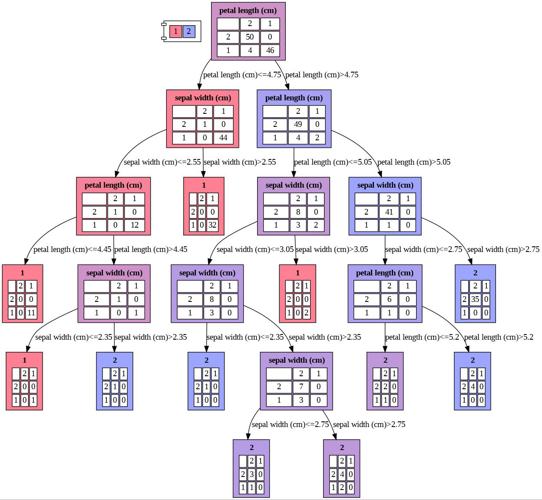
\includegraphics[height=3.5cm, valign=t]{ICC-v1.png}%
           } 
           \subfloat{%
              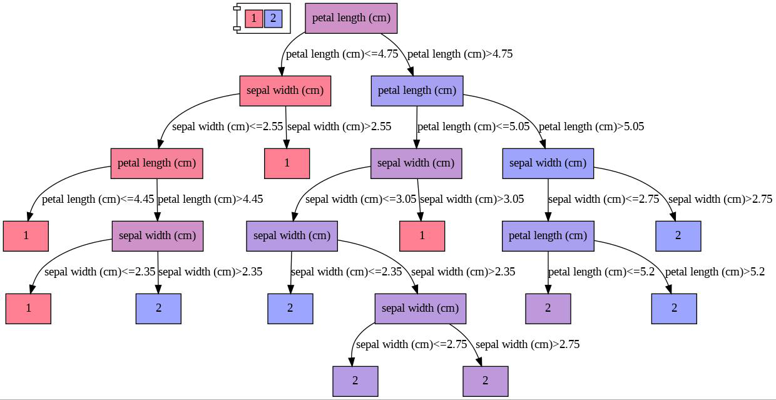
\includegraphics[height=2cm, valign=t]{ICC-v2.png}%
           }
           \subfloat{%
              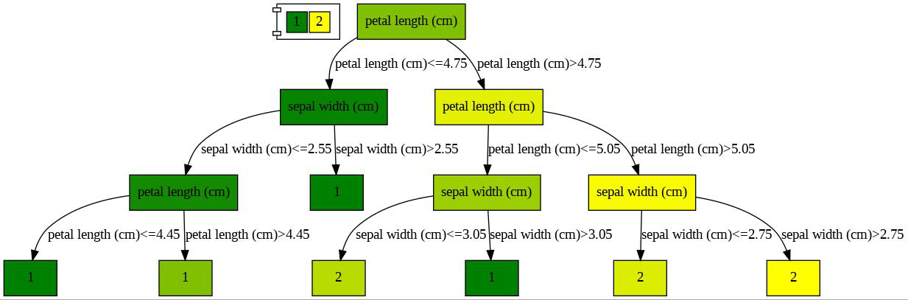
\includegraphics[height=2cm, valign=t]{ICC-v3.png}%
           }
           \caption{Different variations of ICC.}
           \label{fig:fig3}
\end{figure}    


\section{Experimental evaluation}\label{Experimental evaluation}
I evaluated the performance of the ICC plot by comparing it to Scatter and Jitter plots, as a baseline. To do this, I presented four CS students majoring in Data Science two graphs representing different datasets: one Scatter or Jitter plot, and the other - ICC plot.

In the first stage, I asked the students to write down as many observations as possible from each graph. In the second stage, I asked them to determine the relevance of their observations to the classification problem at hand. Finally, I asked them to share the advantages and disadvantages they came across during this evaluation for each graph type.

I repeated this process with three well-known datasets: Iris (to classify iris species), Titanic (to classify survivors and fatalities in the Titanic disaster), and Wisconsin breast cancer data (to classify a cell sample as malignant or benign). 

The results of the first two stages are presented in table 1.\\

\centering
\begin{tabular}{ |m{2cm}|m{6cm}||P{1.9cm}|P{1.9cm}|P{1.9cm}| } 
\hline
\multicolumn{2}{|m{3cm}||}{} & Iris data & Titanic data & Wisconsin breast cancer data \\
\hline
\hline
\multirow{2}{*}{\parbox{4cm}{Scatter\textbackslash\\Jitter plot}} & Mean number of observations according to the graph & 4.25 & 2 & 8.5 \\\cline{2-5}
& Percentage of observations relevant to the classification process &  27.9\% & 50\% & 23.6\% \\
\hline
\multirow{2}{*}{ICC} & Percentage of observations relevant to the classification process & 2 & 2 & 3.5 \\\cline{2-5}
& Percentage of observations relevant to the classification process &  79.1\% & 79.1\% & 75.4\% \\
\hline

\end{tabular}




\section{Related work}\label{Related work}
include a short discussion on relevant existing tools and
techniques. *Cite the works as well as discuss them*. Did they try to
solve the same problem? In what manner your solution different? Did
you use/ got inspiration from it? 

\section{Conclusion}\label{Conclusion}
summarize your finding, and the things you learned from
the project

\bibliographystyle{abbrv}
\bibliography{main}

\end{document}